%! TEX root = /home/duy/TUB/Thesis/latex-source/DiplomarbeitLaTex.tex

\chapter{Evaluation\label{cha:evaluation}}
As we have discussed in the previous chapters, we feed the \acrshort{gan} generated data
to the 2-channel Object Classification network in different proportions with respect to
the amount of original data. On one hand, we expect that \acrshort{gan}, especially the
Generator can be a good data generation engine which can help training the classification
task better. On the other hand, we hope that a well-trained classifier could be a good
tool for quantitatively evaluating \acrshort{gan} data.

In this chapter we describe how we evaluate the data generated from \acrshort{gan} using
such a baseline classifier. The basic idea is to implement the two-channel network from
Eitel et al. and compare the task's performances between using real data and using data
generated from \acrshort{gan}. Different levels of noise injection are also used in order
to evaluate how the baseline task uses depth and RGB information to make decisions.

We train the deep classifier in the following settings:

\begin{itemize}
	\item Using the original data with both Depth and RGB information
	\item Using only a part of the original data (in different scales) with both Depth and
		RGB information
	\item Using a part of the data (in different scales) with both Depth and RGB
		information, the remaining is substituted by \acrshort{gan} generated data
	\item Using the original data but with only RGB information in different scales, which
		is to determine the contribution that Depth data adds to the learning procedure
	\item 
\end{itemize}

\section{Results}
Before going to quantitative measurements, it is worthy to take a look as what our
\acrshort{gan} produces. In Figure~\ref{fig:gan_depth}, 5 random samples from 5 random
categories in the dataset are the outputs from our Depth-GAN in Evaluation Mode, which
means the corresponding \acrshort{gan} did not see those samples in the training process.
The depth maps are all colorized using the jet color-map for visualization purpose. It is
easy to see that the \acrshort{gan} produces very reasonable depth maps with a smooth
range of values. 

Taking a look at those maps, we can see that the \acrshort{gan} does
learn some trivial knowledge. For instance, the bottom pixels tend to be closer to the sensor than the
pixels at the top of the image; and when there is a sharp edge or a sudden change of color
patterns, there is usually an object placed on top of another. We can clearly see the
second property in the sample of an apple and a peach in Figure~\ref{fig:gan_depth}.

In these sample outputs from our Depth-GAN, we also see another popular advantage of
\acrshort{gan} which is already discussed in some other works \cite{gan, cogan, pix2pix}.
That is, the edges in the synthesized images are very sharp. If we instead minimize a
squared loss function for example, we could expect a much more blurry outcome. It is also
one of the reasons that using common scalar error functions such as \acrshort{mse} is not
really a good way to evaluating \acrshort{gan}s' results.

\begin{figure}[h]
	\centering
	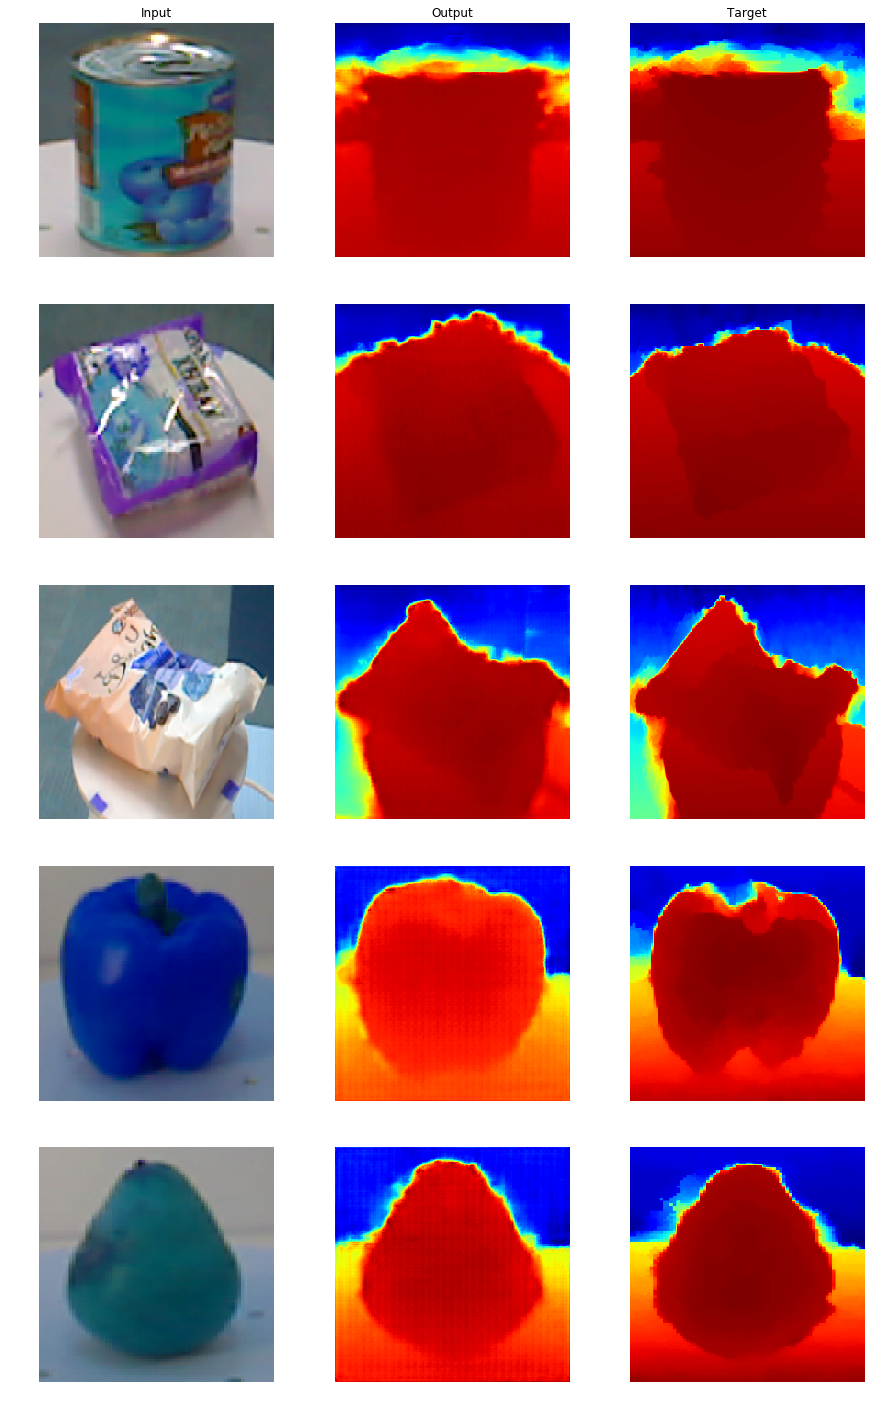
\includegraphics[width=0.75\linewidth]{gan_depth_samples}
	\caption{Some generated samples from Depth-GAN. From Left to Right: Input, Output and
		Target. The \acrshort{gan} reads the Input as a condition and generates the
		Output.  Here the Output and the Target are colorized using the jet color-map. A
		pure red color indicates distance 0 and a pure blue color indicates maximum
	distance from the sensor.}
	\label{fig:gan_depth}
\end{figure}


\section{Accuracies}
In the first experiment, we try to reproduce the paper results \cite{eitel}. We can
see the plotted results in Figure \ref{fig:eitel_accuracies}.

\begin{figure}[h]
	\caption{Classification accuracies on Washington Dataset in different settings,
		trained and tested in 10 stratified random splits. The left number in a pair indicates
		the proportion of real data, and the right number indicates the proportion of synthesized
	data added.}
	\centering
	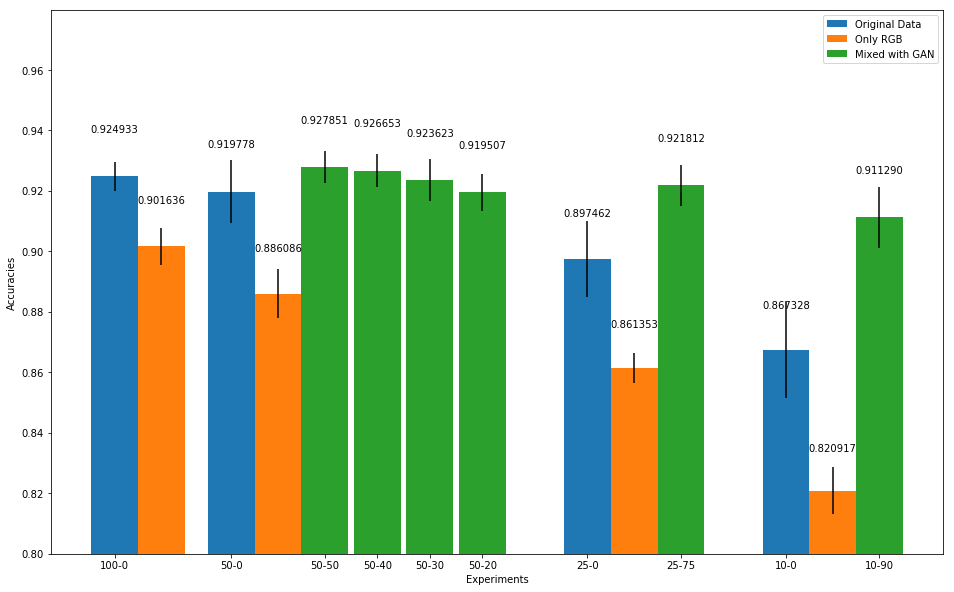
\includegraphics[width=0.75\textwidth]{img/eitel_accuracies}
	\label{fig:eitel_accuracies}
\end{figure}

In general, we can see that \acrshort{gan} has good contribution in the classification
performance. It is worth to mention that the transfer learning technique works very well,
so we still have the accuracies more than 80\% even when we use only 10\% of the data. It
is also expected to see the accuracies drop when we use only RGB data for training the
network, but the difference is only a few percentages, which is an indication that the
contribution of depth information is low in this training procedure. It is not a surprise
because the RGB channels themselves have already achieved a very high accuracy
(approximately 90\%). However, as other works also have shown \cite{eitel, alexandre},
depth information does help improving classification on \acrfull{cnn} when combining with
RGB, our experiment also follows that trend where all the accuracies using depth data are
higher in average than the corresponding results without depth.



\begin{figure}[h]
	\centering
	\begin{subfigure}{0.49\textwidth}
		\centering
		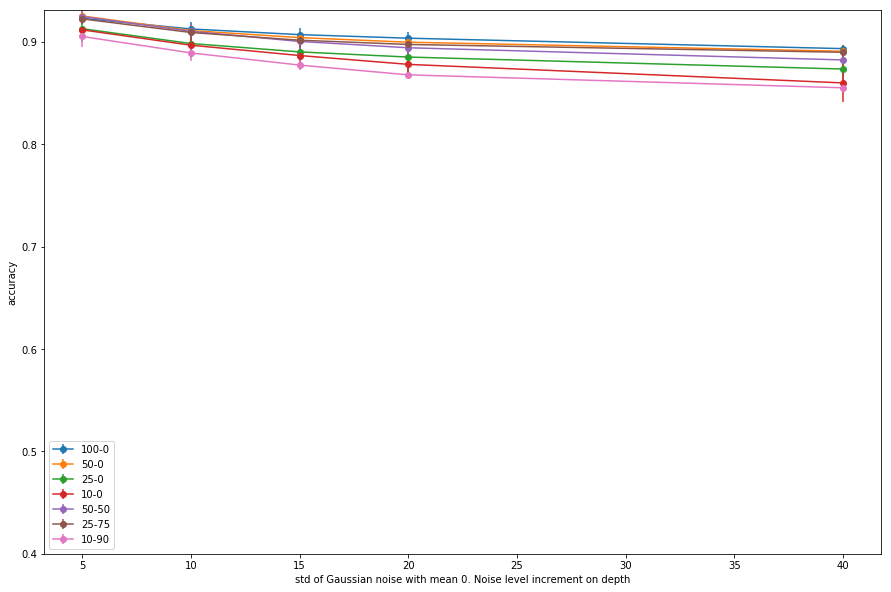
\includegraphics[width=\textwidth]{img/noise_injection_depth}
		\caption{Adding noises to depth}
	\end{subfigure}
	\begin{subfigure}{0.49\textwidth}
		\centering
		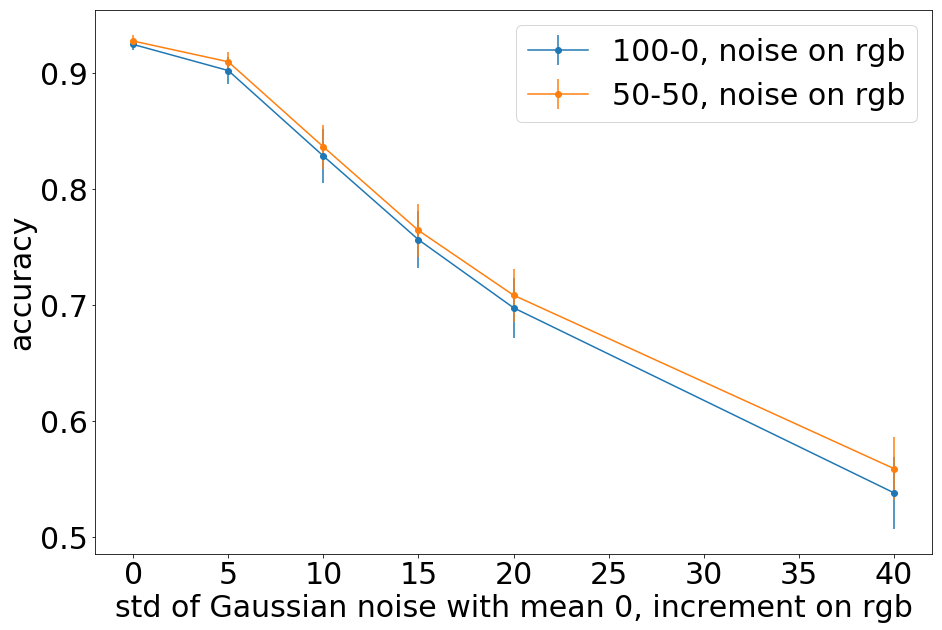
\includegraphics[width=\textwidth]{img/noise_injection_rgb}
		\caption{Adding noises to RGB}
	\end{subfigure}
	\caption{Noise Injection experiment}
	\label{fig:noise_injection}
\end{figure}

